\chapter{Desenvolvimento}

Diferente de muitos outras interfaces de desenvolvimento, o KDEVElop mermiti o usuario incorporar qualquer projeto na IDE,
des de que siga alguns padrões já bem estabelecidos na cultura open source de desenvolvimento de software realizado e C++.
Pois, boa parte das configurações que são buscadas na IDE para a configuração do projeto, vem dos gerenciadores de compilação,
como antes citados, CMAKE e MAKE. Com isso, não é necessario lidar com as burocracias de incorporaçãode projeto, ou até mesmo
o vinculo do projeto a uma certa IDE, impossibilitando o desenvolvimento do mesmo em outros ambiente e fluxos de trabalho.
Os projetos que são realizados com as ferramentas de gerenciamento de compilação, ajuda muito pela sua generalização e
distribuição, por serem projetos de códigos abertos extremamente populares e comuns em projetos de linguagens não interpretadas.

\section{Exposição do tema ou matéria}

Sendo a área de desenvolvimento de sistemas embarcados potencializado nos utlimos anos pela miniaturuzalão do hardware, permitindo
a cada dia um paço mais próximo a um abiente ubiquo com contribuição das bases de desenvolvimento das tecnologias de IoT. Contudo,
como dito anteriormente, os sistemas utilizados atualmente não permitem um fluxo de trabalho agradavel para desevolvedores, muito menos
para empresas de pequeno, médio e até mesmo de grande porte, que se limita as seguintes categorias:

\begin{itemize}
 \item \textbf{Ferramentas proprietárias}: Ferramentas de desenvolvimento para resolver problemas criados pela própria empresa que os fornece, obrigando a utilização de periféricos da mesma distribuidora ou parceira, fazendo limitações de liberdade de desenvolvimento via software. Outras permitem o desenvolvimento limitado a licenças de valores exorbitantes, fazendo com que pequenas empresas que utilizam um baixo capital para se manterem utilizem licenças de baixo custo que limita a utilização do software de maneira praticamente ilegal, como, por exemplo: Pagar uma licença mais cara para utilizar opções de compilação otimizada para uma especifica arquitetura como (-O2 e -OS do GCC) ou até mesmo opções para utilizar o algumas partes do processador (-mfloat-abi e -mfpu dos processadores ARM, permitindo execução de cálculos matricial ou com ponto flutuante em hardware). A utilização de tais ferramentas o majoritariamente usadas comparadas com as demais.
 \item \textbf{Ferramentas gráficas de código aberto}: Utilizadas por uma parte dos desenvolvedores, fornece acesso total ao desenvolvedor do sistema, permitindo modificações e aperfeiçoamentos nos mínimos detalhes do sistema. Estas interfaces permitem o desenvolvimento com uma experiência mais assistencialista, tendo acesso a informações visuais durante o desenvolvimento, como dicas e correções em tempo real, o mais comum entre essas ferramentas, pode-se destacar: corretor de idioma, dicas de autocompletar. menu de seleção de herança ou função de objeto, visualização de documentação da implementação da função, avisos de erro e perigo, entre outros.
 \item \textbf{Ferramentas com \textit{cli}}: Geralmente utilizadas pelas interfaces gráficas como \textit{back-end} para realizar suas
 operações em relação ao sistema embarcado, as ferramentas utilizadas seriam: OpenOCD, Avrdude, esptool, dfu-utils entre outros.
\end{itemize}

\abreviatura{cli}{\textit{Command-line interface}}


\subsection{Ferramentas Utilizadas}
As seguintes ferramentas foram utilizadas para a realização do desenvolvimento do projeto.
\begin{itemize}
 \item \textbf{KDevelop}: Editor de código para programar o plugin e realizar os testes do mesmo nos sistemas embarcados utilizados,
 também utilizado para a realização de debug.
 \item \textbf{Placas de desenvolvimento}: Arduino mini, nano, mega, due, uno para realizar testes no suporte realizado para Arduino
 utilizando avrdude. Stellaris LM4F232 para testes utilizando o suporte feito do OpenOCD.
 \item \textbf{GIT}: Utilizado para realização do controle de versão e documentação do  histórico de desenvolvimento.
 \item \textbf{Astyle}: Ferramenta utilizada para checar e corrigir estilo do código.
 \item \textbf{Codespell}: Script para correção ortográfica da documentação e do código.
 \item \textbf{Doxygen}: Programa assistencialista para geração de documentação.
 \item \textbf{Arch Linux}: Sistema operacional utilizado para realização do desenvolvimento e execução de programas.
 \item \textbf{Valgrind}: Utilizado para realizar a analise de execução do código.
 \item \textbf{KCachegrind}: Ferramenta para visualizar o uso de memória do programa, util para encontrar \textit{memory leaks}.
 \item \textbf{QT Assistant}: Programa assistencialista para visualização a documentação das bibliotecas fornecidades pela QT.
 \item \textbf{QT Designer}: Programa assistencialista para desenvolvimento das interfaces gráficas utilizadas com QT.
 \item \textbf{IRC}: Para retirar duvidas e entrar em contato com outros desenvolvedores do KDevelop.
\end{itemize}

Com o objetivo do trabalho de seguir a filosofia GNU \cite{filosogia}, todos as ferramentas utilizadas para o desenvolvimento do plugin são de código aberto e totalmente gratuitas para qualquer um que queira replicar, modificar e contribuir com o projeto.

\section{Desenvolvimento do software}

\begin{figure}[!htb]
  \centering
  \caption[UML proposto]{UML proposto para desenvolvimento do plugin.}
  \label{fig:uml}
  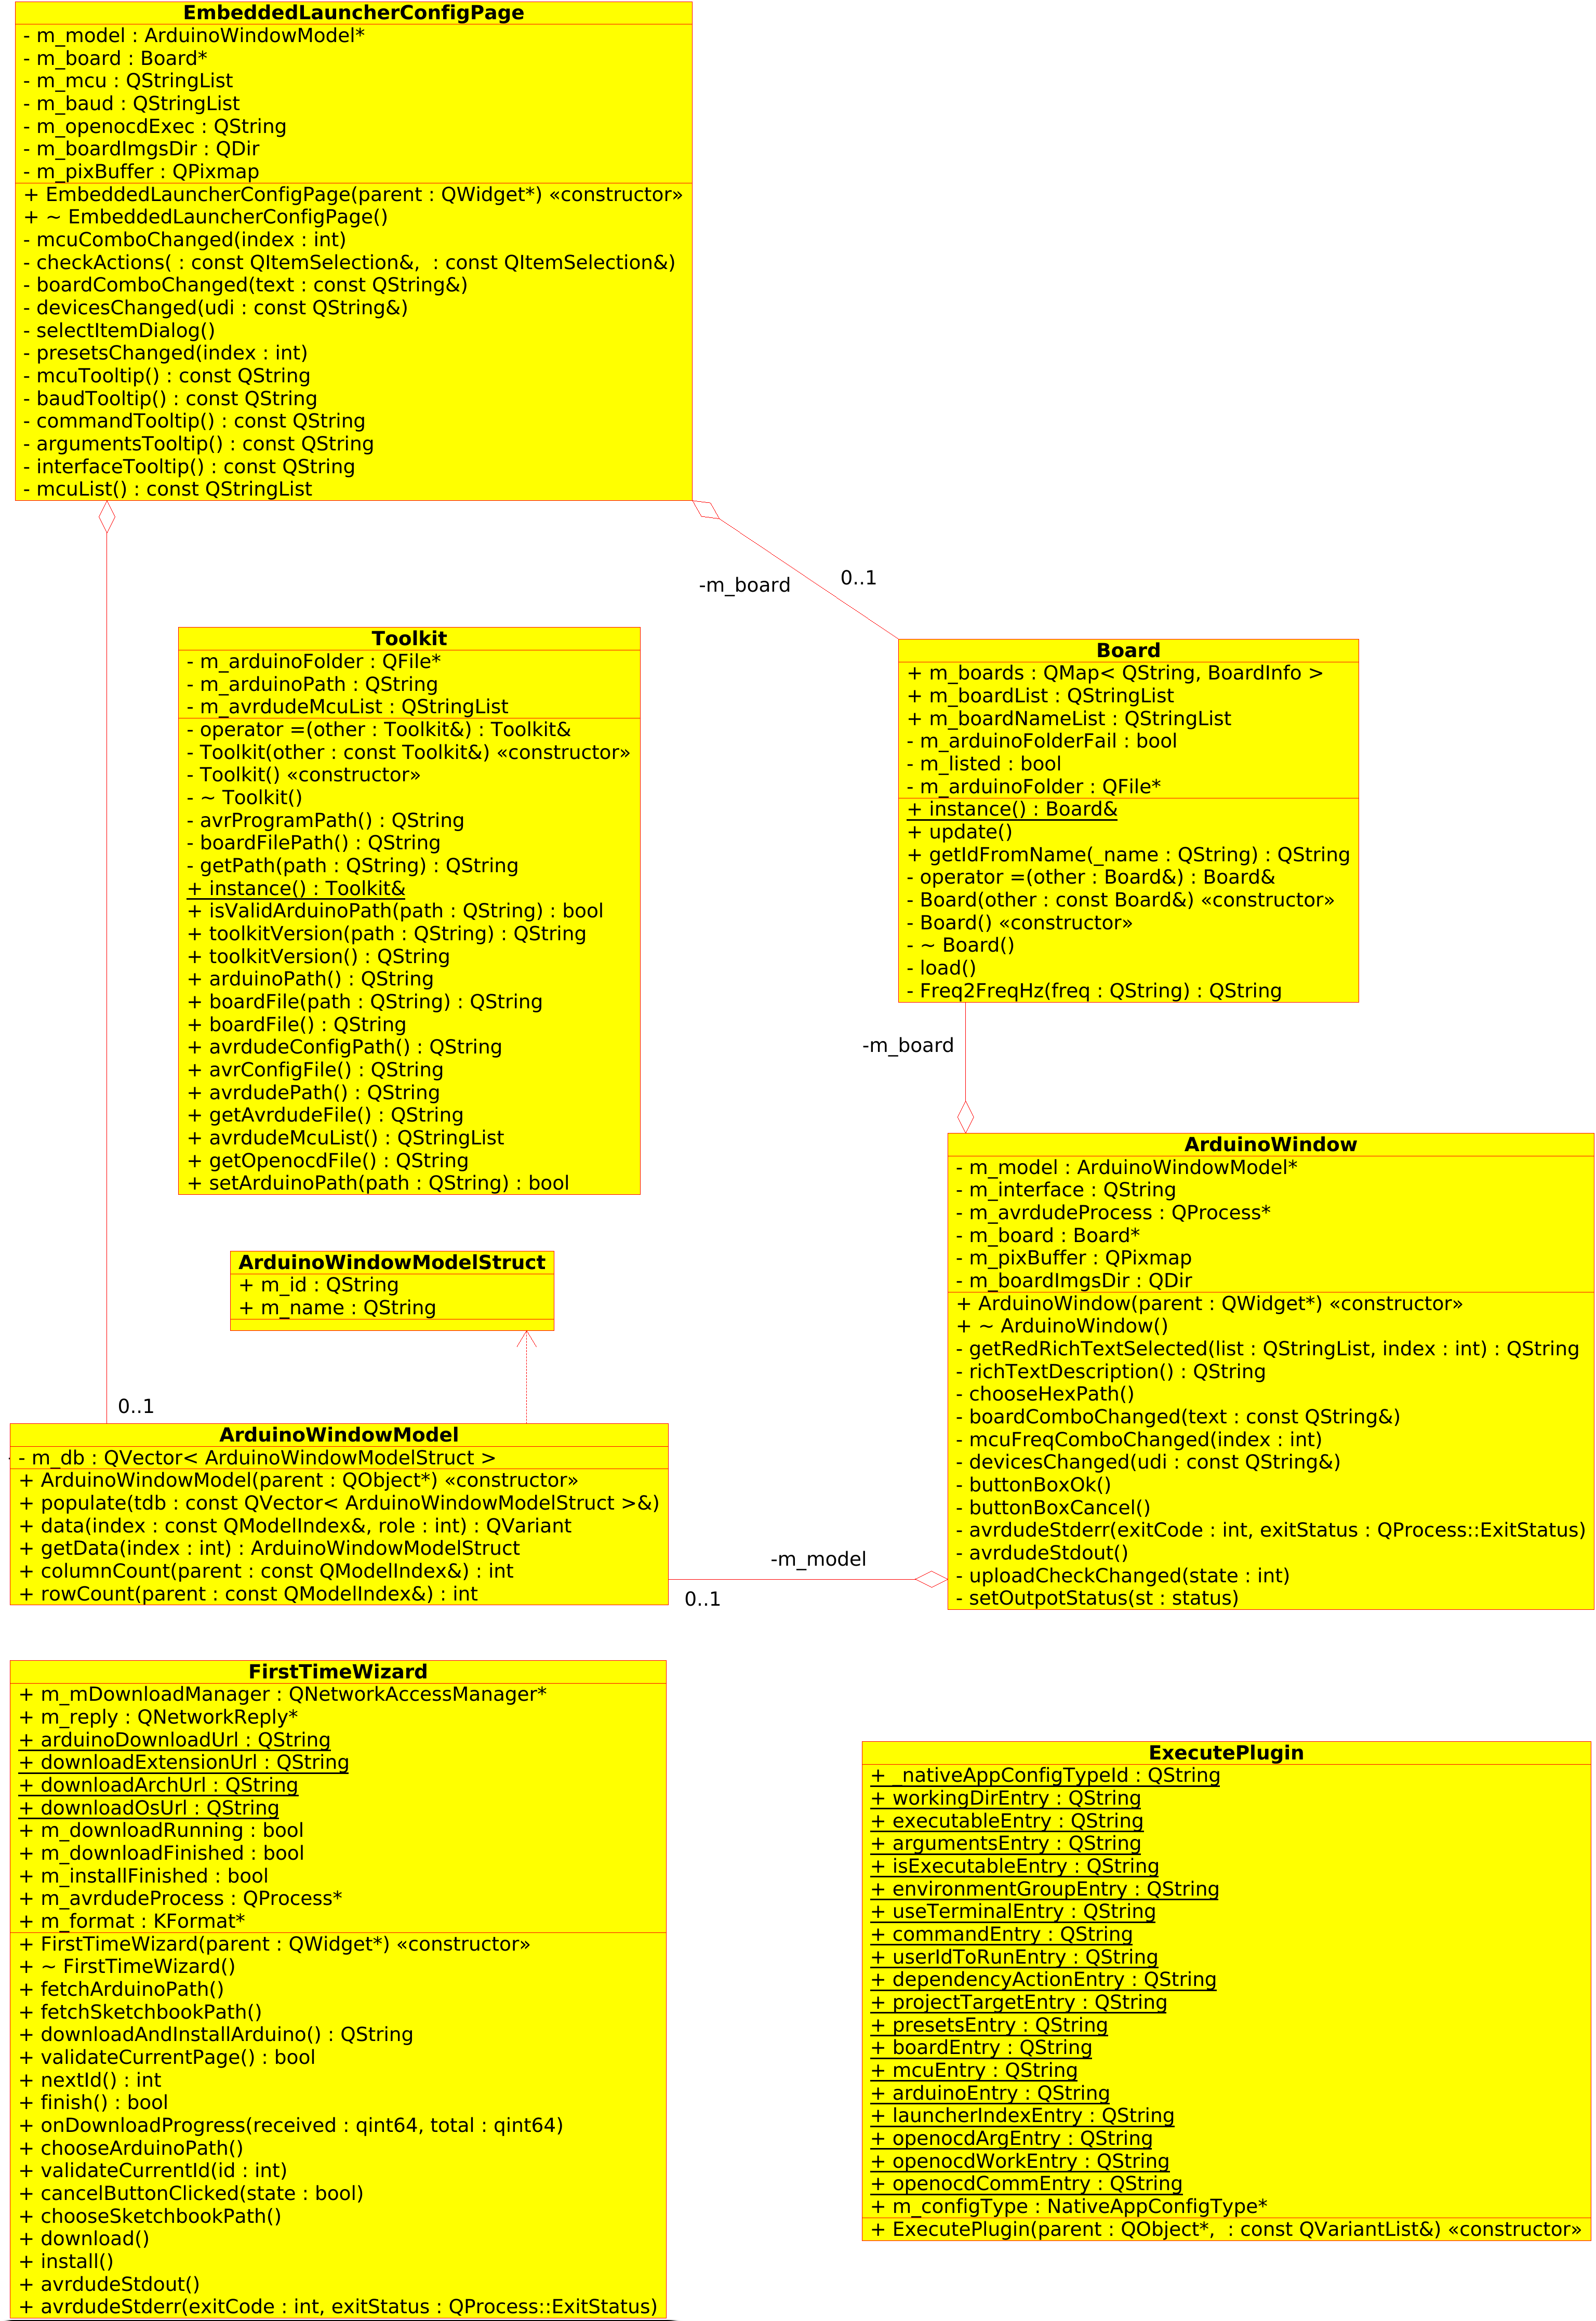
\includegraphics[width=0.85\textwidth]{figuras/uml.png}
\end{figure}

\abreviatura{UML}{Unified Modeling Language}

\section{Integração com KDevelop}

O plugin foi integrado no \textbf{KDevelop} via a utilização de ferramentas básicas de desenvolvimento para o mesmo (\textit{kdevplatform}). Nesta seção, sera posta a amostra as interfaces desenvolvidas e sua integração com o \textbf{KDevelop}, \figref{fig:kdevelop}.

\begin{figure}[!htb]
  \centering
  \caption[KDevelop]{KDevelop após a integração com o plugin proposto.}
  \label{fig:kdevelop}
  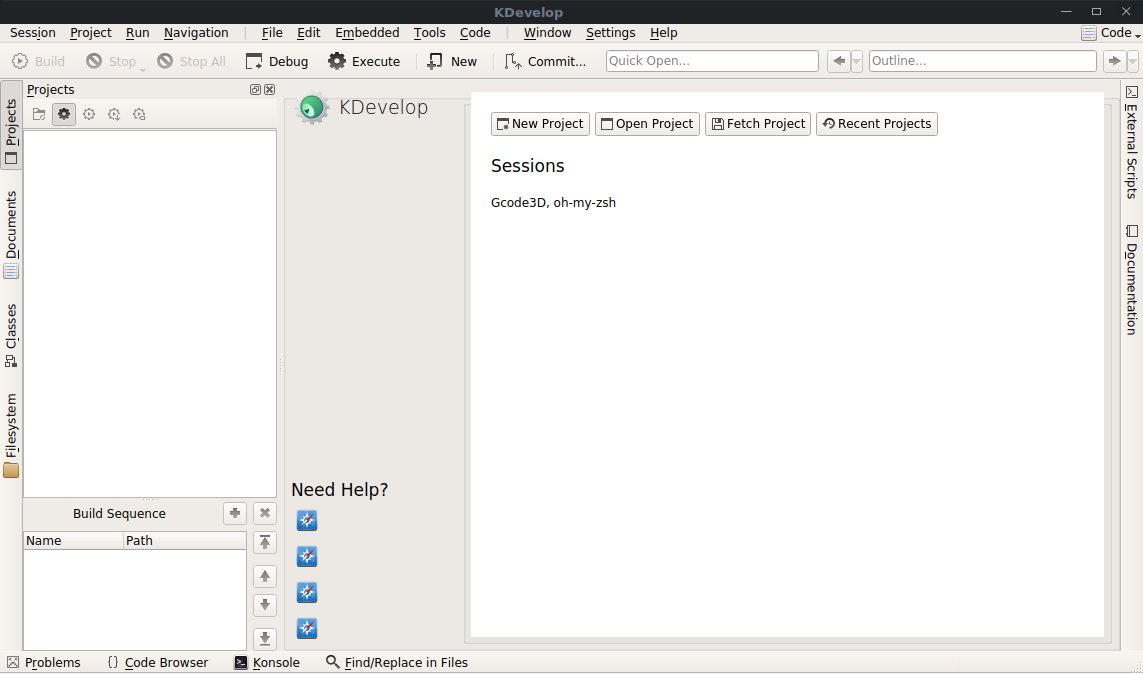
\includegraphics[width=0.85\textwidth]{figuras/kdevelop.png}
\end{figure}

\subsection{Menu de acesso}

O menu de acesso, \figref{fig:kdevelopMenu}, foi desenvolvido para realizar duas principais funções, configurar o plugin em relação as ferramentas necessárias para sua utilização com as placas da \textit{Arduino} (\textbf{\textit{Arduino Setup}}), e permitir a realização de upload do binário desenvolvido para a placa, utilizando uma interface gráfica assistencialista (\textbf{\textit{Board settings}}).

\begin{figure}[!htb]
  \centering
  \caption[Menu do plugin no KDevelop]{Menu de acesso do plugin no KDevelop.}
  \label{fig:kdevelopMenu}
  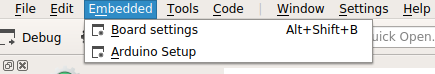
\includegraphics[width=0.95\textwidth]{figuras/kdevelopMenu.png}
\end{figure}

\subsection{Arduino Setup}

Realiza a configuração inicial do plugin no sistema, permitindo o usuário escolher uma versão do \textit{toolkit} do \textit{Arduino} ou fazer com que o plugin realize as instalações necessárias para seu funcionamento.

Primeiramente foi definido um diagrama inicial de estados para facilitar a compreensão da configuração primaria, e como isso serial mostrado para o usuário.

\begin{itemize}
\item \textbf{\textit{First-Time Configuration}}: Tela inicial, permitindo ao usuário escolher o local do \textit{toolkit} previamente instalado (\figref{fig:kdevelopinstaller1}), ou escolher a opção de instalação automática. 

\item \textbf{\textit{Automatic Instalation}}: Tela resultante da escolha da instalação automática na configuração inicial do \textbf{\textit{First-Time Configuration}}. Essa, separada em duas etapas, \textit{Download} e \textit{Install}.

\subitem \textbf{Download}: É realizado a comunicação com o server oficial resultando no \textit{download} do \textit{toolkit}, \figref{fig:kdevelopinstaller21}.

\subitem \textbf{Install}: Após o \textit{download} é realizado a decomposição e instalação do \textit{toolkit}, \figref{fig:kdevelopinstaller22}.

\item \textbf{\textit{End Configuration}}: Tela final, resulta após a escolha de um \textit{toolkit} previamente instalado ou após a conclusão da instalação automática, \figref{fig:kdevelopinstaller3}.
\end{itemize}

O fluxograma destes estados podem ser melhor visualizados na \figref{fig:ftwstate}.

\begin{figure}[!htb]
  \centering
  \caption[Fist-Time Configuration]{Fist-Time Configuration com \textit{Existing Installation} selecionado.}
  \label{fig:kdevelopinstaller1}
  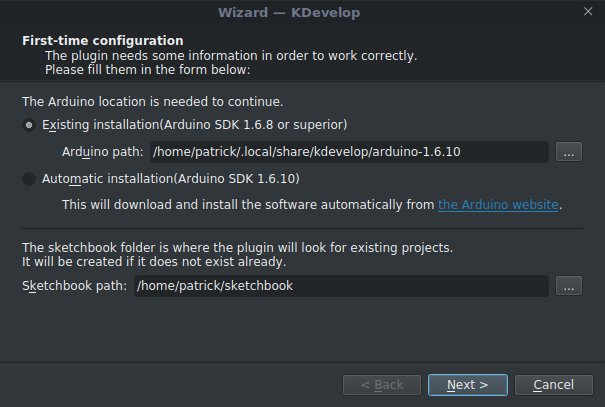
\includegraphics[width=0.95\textwidth]{figuras/kdevelopInstaller1.png}
\end{figure}

\begin{figure}[!htb]
  \centering
  \caption[Automatic Instalation executando Download]{Automatic Instalation com \textit{download} em andamento.}
  \label{fig:kdevelopinstaller21}
  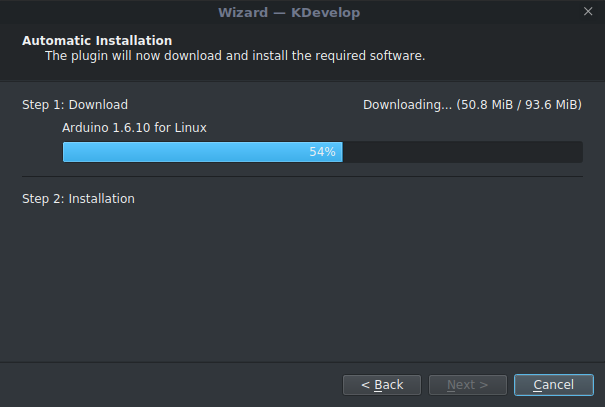
\includegraphics[width=0.95\textwidth]{figuras/kdevelopInstaller21.png}
\end{figure}

\begin{figure}[!htb]
  \centering
  \caption[Automatic Instalation pós instalação]{Automatic Instalation após a instalação do \textit{toolkit}.}
  \label{fig:kdevelopinstaller22}
  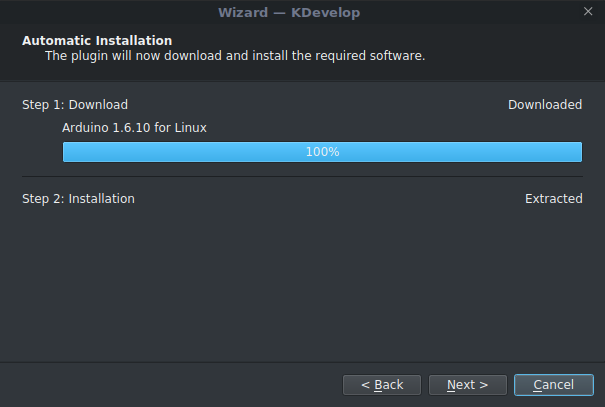
\includegraphics[width=0.95\textwidth]{figuras/kdevelopInstaller22.png}
\end{figure}

\begin{figure}[!htb]
  \centering
  \caption[End Configuration]{End Configuration}
  \label{fig:kdevelopinstaller3}
  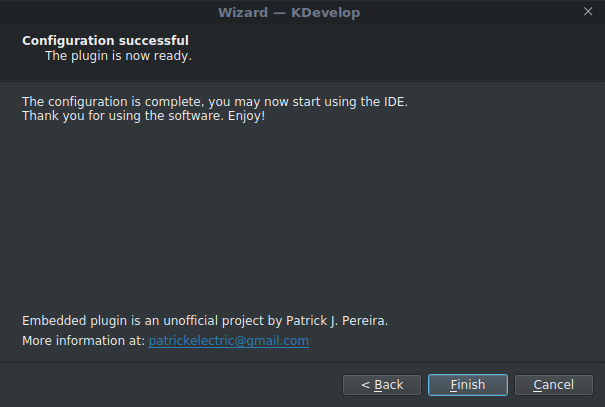
\includegraphics[width=0.95\textwidth]{figuras/kdevelopInstaller3.png}
\end{figure}

\begin{figure*}[ht!]
  \centering
    \caption[Diagrama de estados do \textbf{\textit{First-Time Wizard}}]{\label{fig:ftwstate}}{Diagrama de estados do \textbf{\textit{First-Time Wizard}}}
  \begin{tikzpicture}[->,>=stealth',shorten >=1pt,auto,node distance=2.8cm,semithick]
    \tikzstyle{every state}=[fill=blue,draw=none,text=white]

	%First-Time Configuration
    \node[state]         (A)                    {$FirstTimeConf.$}; 
    % Automactic Install
    \node[state]         (B) [right of=A]       {$Auto Inst.$};
    \node[state]         (C) [right of=B]       {$Down.$};
    \node[state]         (D) [below of=C]       {$Install$};
    \node[state]         (E) [below of=A]       {$EndConf$};

    \path (A) edge              node {Existing Installation}      (E)
	      (A) edge  [bend left]   node {Automatic Installation}      (B)
          (B) edge              node {}      (C)
          (C) edge              node {}      (D)
          (D) edge              node {}      (E);
  \end{tikzpicture}
\end{figure*}




\subsection{Board Settings}

Interface para realizar o envio do binário para o sistema embarcado, permitindo o usuário interagir com o sistema, escolhendo a placa e algumas opções simples como \textit{CPU}, frequência, interface de comunicação, tipo de log de dados da saída do \textit{bootloader}. Além de permitir visualizar e mostrar quais opções foram selecionadas, \figref{fig:boardsettings}.

\begin{figure}[!htb]
  \centering
  \caption[Board Settings com configuração inicial]{Imagem do \textbf{Board Settings} sem configuração prévia.}
  \label{fig:boardsettings}
  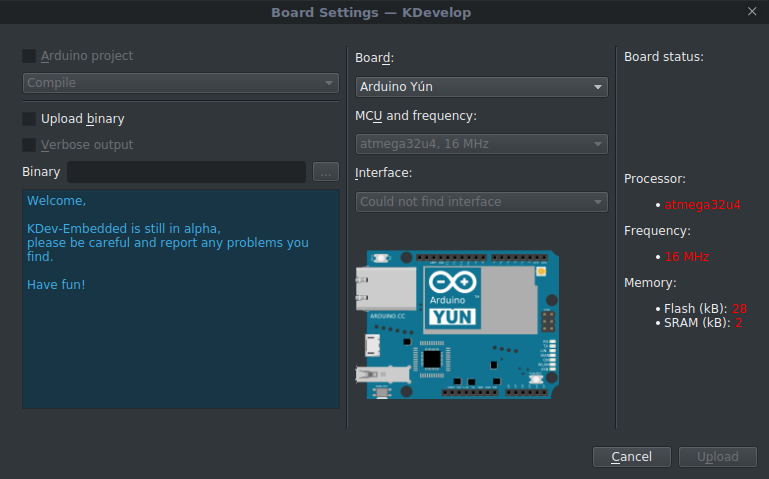
\includegraphics[width=1\textwidth]{figuras/boardsettings.png}
\end{figure}

Após ter o acesso a interface, o usuário pode escolher a opção de \textbf{\textit{Upload Binary}}, selecionado desta forma um arquivo contendo o código de maquina (\textbf{Blink.hex}), após isso, pode escolher no menu \textbf{\textit{Board}} a placa escolhida para programar, permitindo desta forma o plugin selecionar as melhores opções para o hardware selecionado, além disso, é necessário selecionar o tipo de processador e clock, como consta no menu \textbf{\textit{MCU and frequency}}, tendo isto seleciona, a ultima configuração necessária para realizar o envio do código é selecionar a porta que consta no menu \textbf{\textit{interface}} para selecionar o \textit{hardware} de comunicação com a placa. Essas configurações podem ser visualizadas na \figref{fig:boardsettingsserial}, onde foi escolhido um \textbf{Arduino Nano} contendo um processador atmega328p com um clock de $16MHz$ utilizando uma interface de programação \textbf{\textit{FT232 USB UART}}.

\begin{figure}[!htb]
  \centering
  \caption[Board Settings após configuração para envio]{Imagem do \textbf{Board Settings} após configuração do usuário.}
  \label{fig:boardsettingsserial}
  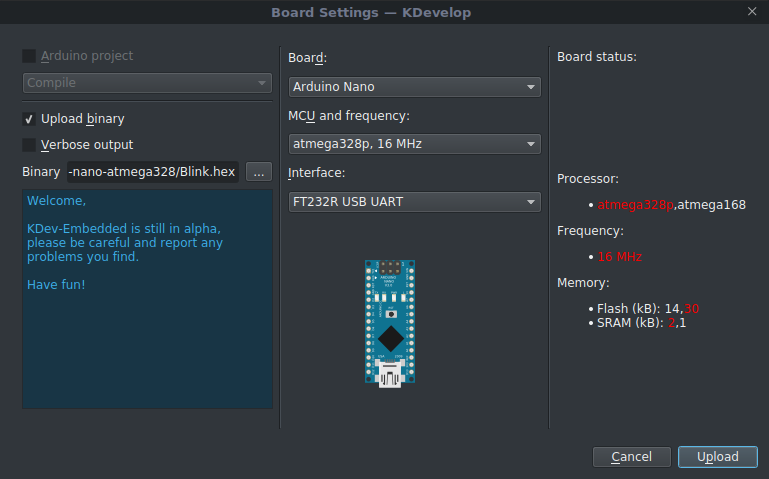
\includegraphics[width=1\textwidth]{figuras/boardsettingsSerial.png}
\end{figure}

Depois de tudo configurado, é possivel clicar no botão \textbf{\textit{upload}} e realizar o envio do binario selecionado para placa. Podendo acarretar no sucesso da operação (\figref{fig:boardsettingsdone}) ou na sua falha (\figref{fig:boardsettingsndone}). Caso a falha aconteça, uma mensagem de erro aparecera juntamente com o código de erro para permitir uma melhor interpretação do problema.


\begin{figure}[!htb]
  \centering
  \caption[Board Settings com sucesso no envio]{Imagem do \textbf{Board Settings} após o envio do código para o sistema embarcado.}
  \label{fig:boardsettingsdone}
  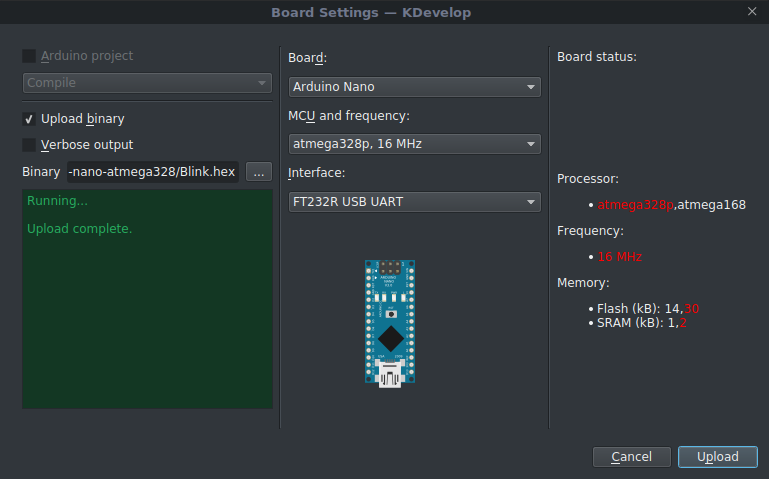
\includegraphics[width=1\textwidth]{figuras/boardsettingsdone.png}
\end{figure}

\begin{figure}[!htb]
  \centering
  \caption[Board Settings com falha no envio]{Imagem do \textbf{Board Settings} após falha no envio do código para o sistema embarcado.}
  \label{fig:boardsettingsndone}
  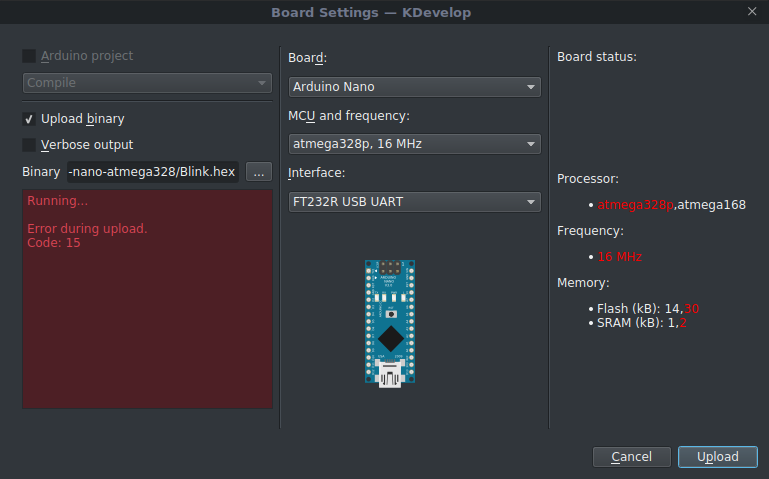
\includegraphics[width=1\textwidth]{figuras/boardsettingsndone.png}
\end{figure}

\section{Integração com fluxo de trabalho}
Além do desenvolvimento do software, permitindo seu uso como projetado inicialmente, foi necessário reservar uma parte do período do projeto para modificações de interface gráfica e de organização de layout, para permitir o uso relativamente simples para usuários não tão avançados, e ao mesmo tempo, permitir uma flexibilidade aos usuários com conhecimento profundo do funcionamento do sistema utilizado no background do projeto\footnote{OpenOCD, avrdude entre outras futuros sistemas opensources que devem ser incorporados no plugin}, modificando e personalizando as opções fornecidas pelo ambiente gráfico sem restringir o alto nível de abstração que essas ferramentas já permitem e prejudicar a liberdade de configurações disponíveis para o usuário.

\subsection{Compilação}

Seguindo o fluxo de trabalho do KDevelop, para se importar um projeto, é necessário realizar a seguinte operação: \textbf{Project $\rightarrow$ Open / Import Project...} e importe um projeto com um sistema de compilação suportado pelo KDevelop, \figref{fig:importproject}.

\begin{figure}[!htb]
  \centering
  \caption[Import Project]{Import Project.}
  \label{fig:importproject}
  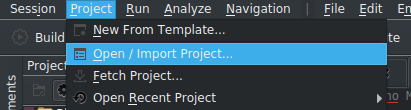
\includegraphics[width=1\textwidth]{figuras/importproject.png}
\end{figure}

Após o projeto ser importado com sucesso, será possível visualizar o mesmo na \textit{dock} de projeto, \figref{fig:projects}.

\begin{figure}[!htb]
  \centering
  \begin{minipage}{.5\textwidth}
  \centering
  \caption[Projects antes da compilação]{Dock Projects antes da compilação do projeto.}
  \label{fig:projects}
  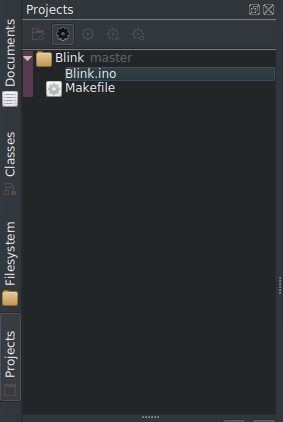
\includegraphics[width=0.7\textwidth]{figuras/projects.png}
  \end{minipage}%
	\begin{minipage}{.5\textwidth}
  \centering
    \caption[Projects depois da compilação]{Dock Projects depois da compilação do projeto.}
  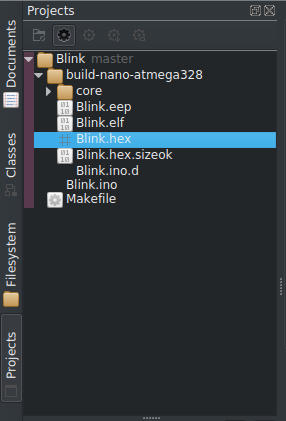
\includegraphics[width=0.713\linewidth]{figuras/projects2.png}
  \label{fig:projects2}
\end{minipage}
\end{figure}

Depois de ter realizado a importação com sucesso, é necessário realizar a compilação do mesmo para gerar o binário que será enviado pro processador, para realizar o processo de compilação, basta clicar no botão \textbf{\textit{Build}} da interface do KDevelop, após isso, o \textit{dock} de projeto se atualizado, podendo ser possível visualizar o arquivo com o código de maquina, \figref{fig:projects2}.

\subsection{Lançamento}

Seguindo o fluxo de trabalho do KDevelop, é necessário configurar o projeto para ser realizado o lançamento de uma forma correta. Para tal, basta ir em \textbf{Run} $\rightarrow$ \textbf{Configure Launchs}, \figref{fig:run}.

\begin{figure}[!htb]
  \centering
  \caption[Configure Launchs]{Configure Launchs.}
  \label{fig:run}
  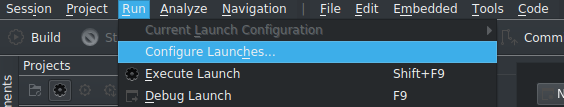
\includegraphics[width=1\textwidth]{figuras/run.png}
\end{figure}

Após isso uma tela de configuração será aberta, podendo ser configurada da seguinte forma para um sistema embarcado, \textbf{Add New...} $\rightarrow$ \textbf{Embedded} e configurar o sistema de acordo com o sistema embarcado que gostaria de ser programado, como pode ser visto na \figref{fig:run2}. Nesta, foi utilizado um \textit{Arduino Nano} para realizar o teste de envio de código, contudo, também é possível utilizar o suporte a \textit{OpenOCD} desenvolvido, \figref{fig:openocd}.

\begin{figure}[!htb]
  \centering
  \caption[Configure Launchs para \textit{avrdude}]{Configure Launchs para \textit{avrdude}.}
  \label{fig:run2}
  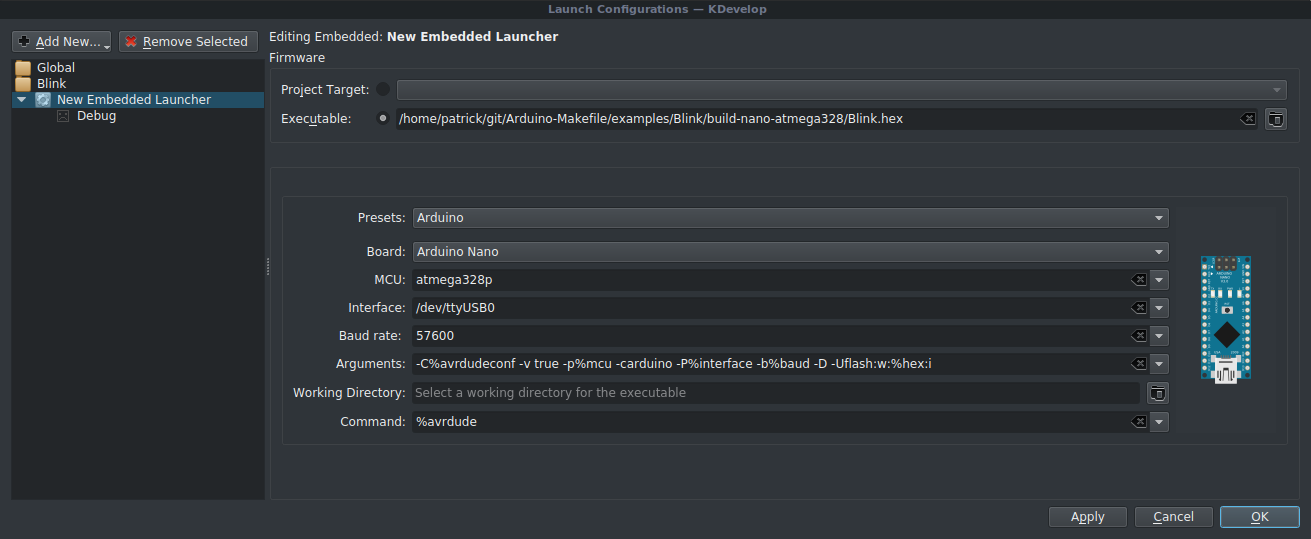
\includegraphics[width=1\textwidth]{figuras/run2.png}
\end{figure}

\begin{figure}[!htb]
  \centering
  \caption[Configure Launchs para \textit{OpenOCD}]{Configure Launchs para \textit{OpenOCD}.}
  \label{fig:openocd}
  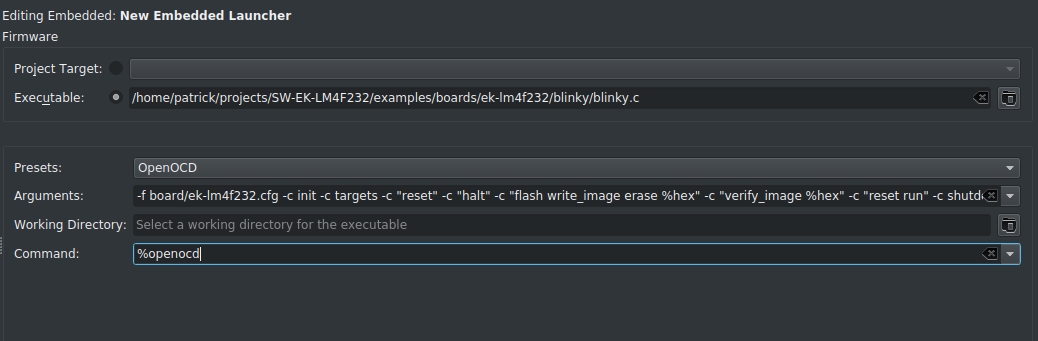
\includegraphics[width=1\textwidth]{figuras/openocd.png}
\end{figure}

Após realizar as configurações, basta aplica-las e em seguida executar o lançamento com o botão \textbf{Execute}. Tendo isso realizado, será aberto um console onde todos os dados de gravação serão mostrados, podendo assim realizar a verificação do funcionamento do sistema, \figref{fig:runavrdude} e \figref{fig:runopenocd}.

Com as configurações salvas no lançador do código, as mesmas ficam reservadas num arquivo conhecido como \textit{*.kdev4}, responsável por gerenciar os arquivos de configuração, logo permitindo que os próximos lançamento sempre utilizem as mesmas configurações, além de permitir outras configurações de lançamento em paralelo.

\begin{figure}[!htb]
  \centering
  \caption[Embedded Launcher com \textit{avrdude}]{Embedded Launcher com saída do \textit{avrdude.}}
  \label{fig:runavrdude}
  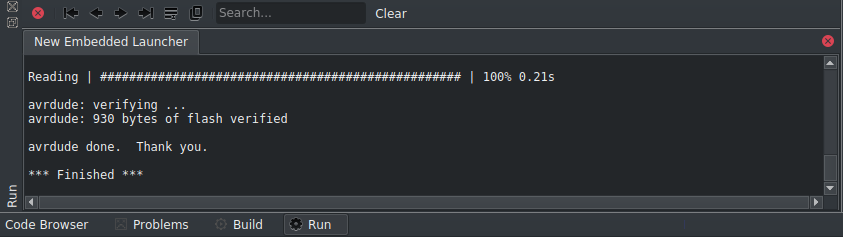
\includegraphics[width=1\textwidth]{figuras/runavrdude.png}
\end{figure}

\begin{figure}[!htb]
  \centering
  \caption[Embedded Launcher com \textit{openocd}]{Embedded Launcher com saída do \textit{openocd.}}
  \label{fig:runopenocd}
  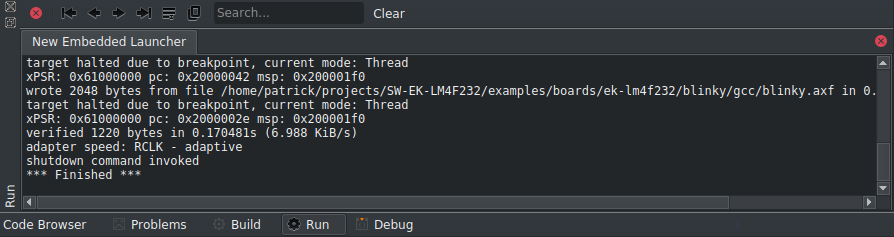
\includegraphics[width=1\textwidth]{figuras/runopenocd.png}
\end{figure}

\subsection{Depuração}

A depuração pode ser utilizada as próprias ferramentas do KDevelop, permitindo uma conexão com o server do GDB pela porta padrão, tal configuração foi testada utilizando a implementação do \textit{OpenOCD}.

